\documentclass[a4paper]{article}
\usepackage{xgreek}
\usepackage[dvipsnames]{xcolor}
\usepackage{xltxtra}
\usepackage{setspace}
\usepackage{graphicx}
\usepackage{listings}
\newcommand{\HRule}{\rule{\linewidth}{0.5mm}}
\newcommand{\tab}{\hspace*{3em}}
\setmainfont[Mapping=TeX-text]{FreeSerif}

\lstset{% general command to set parameter(s)
		% print whole listing small
		basicstyle=\small,
		% underlined bold black keywords
		keywordstyle=\color{Blue}\bfseries,
		% nothing happens
		identifierstyle=,
		% white comments
		commentstyle=\color{white},
		% typewriter type for strings
		stringstyle=\ttfamily,
		% no special string spaces
		showstringspaces=false
		}

\begin{document}
\begin{titlepage}
\begin{center}


\includegraphics[width=0.15\textwidth]{title/Pyrforos2.png}\\[1.cm]
\textsc{\LARGE Εθνικό Μετσόβιο Πολυτεχνείο}\\[1.5cm]

\Large{ Αναφορά Εξαμηνιαίου Project }\\[0.5cm]

% Title
\begin{doublespace}
\HRule \\[0.4cm]
{\huge \bfseries
Βάσεις Δεδομένων
}\\[0.4cm]
Σχεδιασμοί Βάσεων Δεδομένων\\
\end{doublespace}

\HRule \\[1.5cm]

\begin{minipage}{0.4\textwidth}
\begin{flushleft} \large
\begin{tabular}{l l}
Βασίλης \textsc{Γερακάρης} & (08092)\\
Διονύσης \textsc{Ζήνδρος} & (06601)\\
Γρηγόρης \textsc{Λύρας}	& (09687)\\
\end{tabular}
\end{flushleft}
\end{minipage}
\begin{minipage}{0.4\textwidth}
\begin{flushright} \large
\emph{Διδάσκοντες:} \\
Γιάννης \textsc{Βασιλείου}\\
Τίμος \textsc{Σελλής}
\end{flushright}
\end{minipage}

\vfill

{\large \today}
\end{center}
\end{titlepage}



%{{{ Λεπτομέρειες Υλοποίησης

\section{Λεπτομέρειες Υλοποίησης}

Το project κατασκευάστηκε ως μια εφαρμογή ιστού, με έμφαση στην χρηστικότητα
των ιστοσελίδων και την εύκολη πρόσβαση στα δεδομένα.

Για την υλοποίηση του χρησιμοποιήθηκε το \emph{LAMP} stack δηλαδή:
\begin{itemize}
\item GNU-\textbf{L}inux (διανομή Debian squeeze ως λειτουργικού συστήματος)
\item \textbf{A}pache (Web Server)
\item \textbf{M}ySQL (DataBase Management System)
\item \textbf{P}HP (Scripting Language).
\end{itemize}
Ως database (storage) engine επιλέχθηκε η InnoDB.
Επιπλέον, έγινε χρήση CSS για επεξεργασία της μορφοποίησης των ιστοσελίδων,
και JavaScript.\\
Όλο το προαναφερθέν λογισμικό είναι ανοιχτού κώδικα (open source).\\

Κατα τη φάση σχεδίασης, αποφασίστηκε η εφαρμογή της αρχιτεκτονικής \emph{MVC}
(\textbf{M}odel/\textbf{V}iew/\textbf{C}ontroller), η οποία ορίζει σαφή
διαχωρισμό μεταξύ των διαφόρων συνιστωσών της εφαρμογής.

Έτσι το project αναλύθηκε σε \underline{models}, οπου εμπεριέχεται όλη η λογική
επικοινωνίας με τη βάση, \underline{views}, όπου γίνεται η παραγωγή της διεπαφής
με το χρήστη, και \underline{controllers}, όπου αποφασίζεται ποιο view και model
θα κληθεί, και υλοποιεί τη σωστή επικοινωνία μεταξύ τους.\\

Με τον τρόπο αυτό, καθίσταται ευκολότερη και ταχύτερη η ανάπτυξη και η
αποσφαλμάτωση του λογισμικού, ενώ ο κώδικας είναι πιο ευέλικτος, αφού
αποκρύπτονται οι λεπτομέρειες υλοποίησης μεταξύ των συνιστωσών (αγνωστικό
μοντέλο - αποσύνδεση).

\subsection{Πλεονεκτήματα}
Η επιλογή του παραπάνω τρόπου υλοποίησης επιφέρει αρκετά πλεονεκτήματα, τα
σημαντικότερα των οποίων είναι τα παρακάτω:

\begin{itemize}
\item Η κατασκευή σε μορφή ιστοσελίδων επιτρέπει πρόσβαση στη βάση από
οποιονδήποτε υπολογιστή, χωρίς να εμφανίζονται διαφορές από όσους
χρησιμοποιούν διαφορετικά λειτουργικά συστήματα.
\item Η διανομή Debian squeeze (stable) διακρίνεται για τη σταθερότητα και την
ασφάλειά που προσφέρει, επομένως είναι ιδανική για μια εφαρμογή web server.
\item Εύκολη σύνταξη κώδικα, λόγω της ομαλής καμπύλης εκμάθησης της PHP και της
MySQL
\item Εύκολη ανάπτυξη λογισμικού, αφού τα αρχεία της PHP αποθηκεύονται
και επεξεργάζονται απευθείας σε remote Web server, κάτι που μας επέτρεψε
απομακρυσμένη και ταυτόχρονη πρόσβαση και εργασία.
\item Εύκολη κατασκευή της διεπαφής με το χρήστη με χρήση ιστοσελίδων.
\item Αξιόπιστες συναλλαγές με τη βάση, αφού το InnoDB ικανοποιεί τις ιδιότητες
\emph{ACID} (\textbf{A}tomicity, \textbf{C}onsistency, \textbf{I}solation,
\textbf{D}urability).
\item Γρήγορη (σχεδόν άμεση) ανάκαμψη από crashes ή μη-αναμενόμενα shutdowns,
αφού το InnoDB απλώς επαναλαμβάνει της ενέργειες στα log files της, αντίθετα με
το MyISAM, που ελέγχει και επισκευάζει όλους τους δείκτες και πίνακες.
\end{itemize}

\subsection{Μειονεκτήματα}
Οι επιλογές μας είχαν και τα μειονεκτήματά τους, όπως αναφέρονται παρακάτω:

\begin{itemize}
\item Η MySQL δεν υποστηρίζει constraint checking, οπότε οι περιορισμοί που
θέλαμε να υπάρχουν εφαρμόστηκαν στην host γλώσσα, και απλώς αναφέρονται στα
DDL κατασκευής της βάσης για λόγους πληρότητας.
%TODO - Σκέφτεται κανείς κάτι άλλο?
\end{itemize}

%}}}

%{{{ Σχεδιασμός βάσης

\section{Σχεδιασμός Βάσης}

Για την υλοποίηση της βάσης μας, χρησιμοποιήσαμε το σχεσιακό μοντέλο, όπως το
δημιουργήσαμε για την 1\textsuperscript{η} άσκηση του μαθήματος (όπου
αναλύονται και σε μεγαλύτερο βάθος οι επιλογές και οι παραδοχές μας.

Το σχήμα του relationship model, παρατίθεται παρακάτω:

\begin{figure}[h]
\centering
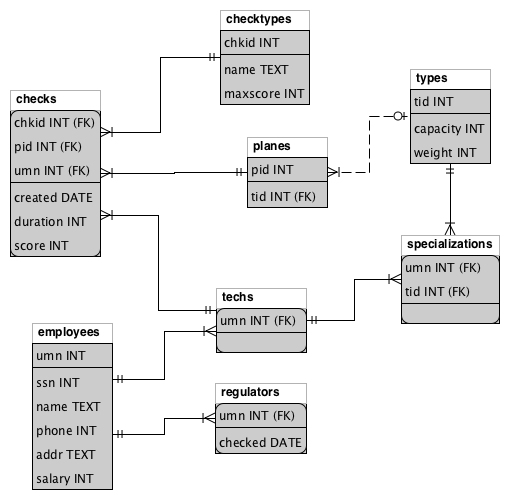
\includegraphics[width=0.9\textwidth]{files/r-db.png}
\caption{Διάγραμμα σχεσιακού μοντέλου}
\end{figure}

Στη σχεδίαση αυτή, προσθέσαμε ορισμένους περιορισμούς, οι οποίοι προκύπτουν
λογικά και υλοποιήθηκαν με check constraints στη MySQL. Αυτοί είναι:

\begin{itemize}
\item Σε όσες σχέσεις χρησιμοποιούν ξένα κλειδιά, υπάρχουν συνθήκες 'ON
DELETE' και 'ON UPDATE' που πραγματοποιούν μια ενέργεια (συνήθως CASCADE).
\item Στην τιμή score του πίνακα checks υλοποιήθηκε check ώστε να έχει τιμή
όχι μεγαλύτερη από το maxscore του αντίστοιχου checktype.
\end{itemize}

Εκτός αυτών, για πληθώρα πεδίων που θα πρέπει να είναι μη αρνητικά,
χρησιμοποιήθηκε ως datatype το unsigned int, ώστε να μη συνταχθούν αχρείαστα
constraints.

Όπως αναφέραμε, η MySQL δεν υποστηρίζει constraint checking, επομένως οι
περιορισμοί υλοποιήθηκαν στην host γλώσσα (php) με χρήση φίλτρων, όπου
χρειάστηκαν, εώς ότου υπάρξει υποστήριξη από το DBMS.

%}}}

%{{{DDL script
\section{DDL Script κατασκευής βάσης}
Παρατίθεται το DDL script που χρησιμοποιήθηκε για να κατασκευαστεί η βάση:

\lstinputlisting[language=SQL]{files/aviation.sql}

Παραπάνω, φαίνεται και η κατασκευή του view "workers", το οποιό αντιστοιχίζει
σε κάθε εργαζόμενο την ιδιότητά του (και χρησιμοποιήθηκε αργότερα για την
εξαγωγή στατιστικών των εργαζομένων). Επίσης, φαίνεται και η χρήση nested
query, προκειμένου να οριστεί ο περιορισμός του πεδίου score από το maxscore
του αντίστοιχου ελέγχου.

%}}}

%{{{SQL queries and Views

\section{SQL queries}
Σε όλες τις σχέσεις της βάσεις μας έχουν δημιουργηθεί queries για εισαγωγή,
ενημέρωση, διαγραφή και επιλογή μίας ή όλων των εγγραφών, τα οποία δε χρειάζονται
καμία εξήγηση.

\subsection{Εργαζόμενοι}
Στους εργαζόμενους έχουμε το 1ο ερώτημα με συναθροιστική συνάρτηση καθώς και
ομαδοποίηση, που μας επιστρέφει τον ελάχιστο, μέσο και μέγιστο μισθό για κάθε
απασχόληση.
    \lstinputlisting[language=SQL]{files/employee.sql}
\subsection{Τύποι Αεροσκαφών}
    \lstinputlisting[language=SQL]{files/planetype.sql}
\subsection{Αεροσκάφη}
H επιλογή των planes, χρησιμοποιεί INNER JOIN με τα planetypes, προκειμένου να
εμφανίσουμε πληροφορίες σχετικά με το αεροπλάνο.\\
Υπάρχει και ένα aggregate query όπου καταμετράται το πλήθος των αεροσκαφών που
υπάρχουν για κάθε δεδομένο planetype.
    \lstinputlisting[language=SQL]{files/plane.sql}
\subsection{Ελεγκτές Εναέριας Κυκλοφορίας}
    \lstinputlisting[language=SQL]{files/regulator.sql}
\subsection{Τεχνικοί}
    \lstinputlisting[language=SQL]{files/tech.sql}
\subsection{Ειδικότητες}
Στις επιλογές των specializations πραγματοποιούνται inner joins με τους
πίνακες employees και planetypes, προκειμένου να εμφανίσουμε χρήσιμες
πληροφορίες.
    \lstinputlisting[language=SQL]{files/specialization.sql}
\subsection{Έλεγχοι}
	Η επιλογή στους ελέγχους πραγματοποιεί CROSS JOIN με 4 διαφορετικές
	σχέσεις, προκειμένου να αντλήσουμε όλες τις πληροφορίες που θεωρήσαμε
	χρήσιμες για το χρήστη.\\
	Επιπλέον, υπάρχει και ένα query ομαδοποίησης με περιορισμό (GROUP BY /
	HAVING) όπου μας εμφανίζονται τα ελαττωματικά αεροσκάφη, δηλαδή αυτά που
	έχουν συνολική επίδοση κάτω από 50\% στους ελέγχους που έχουν υποβληθεί.
    %TODO FIX THIS FILE GREG \lstinputlisting[language=SQL]{files/checks.sql}
\subsection{Αρχεία Εικόνων}
    \lstinputlisting[language=SQL]{files/image.sql}

%}}}

\end{document}
